
\chapter{Decision trees for classification}

So far our classification picture has been very general. We haven't said
anything about how our classifier might actually \textit{work}; we've just said
that given values for each of the features, it will render a prediction about
what the label will be.

\index{decision tree}

In this chapter, we'll study one particular algorithm for classification in
machine learning: the \textbf{decision tree} algorithm.

\section{A working example}

\index{catalog} \index{videogames}
Here's a (fictitious) domain problem that we'll use to demonstrate the
principles in this chapter. Say we own a videogame business, and we want to
send full-color product catalogs to unsuspecting college students, so that they
will buy our games and keep us in business (while meanwhile failing out of
school due to playing all the time).

Now full-color catalogs are expensive to print and ship, so we want to be smart
about this. We definitely don't want to send a bunch of catalogs to students
who aren't likely buyers; that would run our business into the ground. Instead,
we'd like to identify the subset of students who probably gamers, and send
catalogs to only \textit{those} students.

Suppose that through nefarious means, we have acquired the following data set:

\begin{Verbatim}[fontsize=\small,samepage=true,frame=single,framesep=3mm,xleftmargin=4.3cm,xrightmargin=4.2cm]
   major  age gender   VG
0   PSYC   22      F   No
1   MATH   20      F   No
2   PSYC   19      F   No
3   CPSC   20      M  Yes
4   MATH   18      M  Yes
5   CPSC   20      F   No
6   CPSC   19      O   No
7   CPSC   17      M  Yes
8   PSYC   18      F   No
9   CPSC   20      F   No
10  MATH   18      F   No
11  CPSC   22      F  Yes
12  MATH   21      M   No
13  CPSC   23      M  Yes
14  PSYC   17      M  Yes
15  CPSC   18      F   No
16  PSYC   19      F  Yes
\end{Verbatim}

\index{Psychology}
\index{Mathematics}
\index{Computer Science}

Each row represents one college student, with three features. The first is
their major -- \texttt{PSYC} (Psychology), \texttt{MATH} (Mathematics), or
\texttt{CPSC} (Computer Science). (For simplicity, we'll say these are the only
three possibilities, since your author happens to like them the best.) The
second is their age (numeric), and the third is their gender: male, female, or
other. The last column is our target: \textit{whether or not this student is a
videogamer.} Glance over this \texttt{DataFrame} for a moment.

\subsection{Eyeing the prior}

\index{value\_counts@\texttt{.value\_counts()} method (Pandas)}

As you remember from section~\ref{prior}, before we even think about features,
we might as well the target variable itself, and ask ourselves ``given no other
information about a student, what would be our gut feel about their videogame
status?'' Our pal the \texttt{.value\_counts()} method is perfect to compute
this:

\begin{Verbatim}[fontsize=\small,samepage=true,frame=single,framesep=3mm]
print(students.VG.value_counts())
\end{Verbatim}
\vspace{-.2in}

\begin{Verbatim}[fontsize=\small,samepage=true,frame=leftline,framesep=5mm,framerule=1mm]
N    10
Y     7
Name: VG, dtype: int64
\end{Verbatim}

So if we're smart, we'd guess ``no'' for such mysterious persons, but we could
only expect to be right about $\frac{10}{17}^\textrm{ths}$, or 59\%, of the
time.

\subsection{Sticking with categorical features}

\index{categorical variable}

Now it turns out that decision trees work best with all categorical features,
not a mix of categorical and numeric. So for now, we're going to simply
classify each of our students into three buckets: ``\texttt{young}'' (18 or
younger), ``\texttt{middle}'' (19-21), and ``\texttt{old}''
(22+).\footnote{\index{Swift@Swift, Taylor} Believe it or not, a time will come in
your life when 22 years of age does not remotely seem ``old.'' For undergrads,
though, I can see why 22 would seem on the grey side, Taylor Swift's song
notwithstanding.} For the moment, don't ask why we chose three age categories
instead of two or four, and don't ask why we chose those particular split
points. We just did. More on that later.

Our training data now looks like this:

\begin{Verbatim}[fontsize=\small,samepage=true,frame=single,framesep=3mm,xleftmargin=4cm,xrightmargin=4cm]
   major     age gender   VG
0   PSYC     old      F   No
1   MATH  middle      F   No
2   PSYC  middle      F   No
3   CPSC  middle      M  Yes
4   MATH   young      M  Yes
5   CPSC  middle      F   No
6   CPSC  middle      O   No
7   CPSC   young      M  Yes
8   PSYC   young      F   No
9   CPSC  middle      F   No
10  MATH   young      F   No
11  CPSC     old      F  Yes
12  MATH  middle      M   No
13  CPSC     old      M  Yes
14  PSYC   young      M  Yes
15  CPSC   young      F   No
16  PSYC  middle      F  Yes
\end{Verbatim}

and we're now officially ready to consider decision trees.

\section{Decision Trees}

\index{decision tree}
\index{root (of a decision tree)}

First, let's get our head around what a decision tree \textit{is}. Our
inaugural example is shown in Figure~\ref{fig:decisionTree}. The first thing
you'll notice is that it has a branching structure that branches...down. I'm
not sure why Data Scientists draw trees growing \textit{down} while the rest of
the world (including trees themselves: go ahead and look outside) grow up, but
this is the convention so we'll just deal with it. To make it even more
comical, the oval at the top of the tree is called the \textbf{root} of the
tree. Really.

\begin{figure}[ht]
\centering
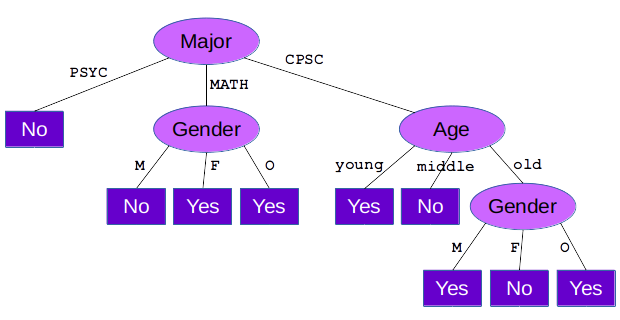
\includegraphics[width=0.9\textwidth]{decisionTree.png}
\caption{A decision tree (not a particularly good one, as it'll turn out) for
the videogame data set.}
\label{fig:decisionTree}
\end{figure}

\index{branch (of a decision tree)}
\index{leaf (of a decision tree)}
\index{node (of a decision tree)}

Continuing full bore with the botany analogy, the lines connecting the various
shapes are, as you might suspect, called \textbf{branches}, and the darker
rectangles are called \textbf{leaves}. One non-botanic bit of lingo is the name
for the other ovals: they're called \textbf{nodes}.

\subsection{Classifying with a decision tree}

Okay. Now what does a decision tree ``mean?'' Geekily-put, it's the pictorial
codification of an algorithm for classification. Not so geekily, it's a map
that tells your classifier what rules to follow as it forms its prediction for
an example data point.

You simply start at the root, considering feature values at each node, and
following the matching branch down the tree. When you reach a leaf, the
prediction you give is written on the leaf node. It's that simple.

\begin{itemize}

\item[\leftpointright] First example: suppose we have a 24-year-old male
Psychology major. We want to know whether he's likely to play videogames. The
decision tree in Figure~\ref{fig:decisionTree} tells us to first consider his
\textsf{major}. Since this is \texttt{PSYC}, we're done: we're immediately at a
leaf. Our prediction for this guy is \texttt{No}, he probably doesn't play
videogames.

\item[\leftpointright] Second example: we have an 18-year-old Math major who
doesn't identify with either of the binary genders. Starting again at the root,
we now follow the middle branch for \texttt{MATH}. Now, we look at the person's
gender. Since it is \texttt{O}, we follow the right branch, and give a
prediction of \texttt{Yes}, we predict they \textit{do} play videogames.

\item[\leftpointright] Third example: we now have a 22-year-old female Computer
Science major. Do we think she would play videogames? The root tells us to look
at her \textsf{major} first, which means we go right; then we look at her
\textsf{age}, and since she's positively ancient we go right again; and
finally, her \textsf{gender} tells us to predict \texttt{No}, she's probably
not a gamer.

\end{itemize}

Most students find this interpretation very straightforward.

\subsection{Decision Trees in Python}

\index{nested if statements@nested \texttt{if} statements}
\index{indentation}

Now to actually automate something, of course, we write code rather than draw
pictures. What would Figure~\ref{fig:decisionTree} look like in Python code?
It's actually pretty simple, although there's a lot of nested indentation. See
if you can follow the flow in Figure~\ref{fig:pythonDT}.

\begin{figure}[h]
\centering
\begin{Verbatim}[fontsize=\footnotesize,samepage=true,frame=single,framesep=3mm,xleftmargin=2cm,xrightmargin=2cm]
def predict(major, age, gender):
    if major == 'PSYC':
        return 'No'
    elif major == 'MATH':
        if gender == 'M':
            return 'No'
        elif gender == 'F':
            return 'Yes'
        elif gender == 'O':
            return 'Yes'
    elif major == 'CPSC':
        if age == 'young':
            return 'Yes'
        elif age == 'middle':
            return 'No'
        elif age == 'old':
            if gender == 'M':
                return 'Yes'
            elif gender == 'F':
                return 'No'
            elif gender == 'O':
                return 'Yes'
\end{Verbatim}
\caption{A Python implementation of the decision tree in
Figure~\ref{fig:decisionTree}.}
\label{fig:pythonDT}
\end{figure}

\index{predict@\texttt{predict()}}

We're defining a function called \texttt{predict()} that takes three arguments,
one for each feature value. The eye-popping set of
\texttt{if}/\texttt{elif}/\texttt{else} statements looks daunting at first, but
when you scrutinize it you'll realize it perfectly reflects the structure of
the purple diagram. Each time we go down one level of the tree, we indent one
tab to the right. The body of the ``\texttt{if major == 'PSYC':}'' statement is
very short because the left-most branch of the tree (for Psychology) is very
simple. The ``\texttt{elif major == 'CPSC':}'' body, by contrast, has lots of
nested internal structure precisely because the right-most branch of the tree
(for Computer Science) is complex. \textit{Etc.}

\begin{samepage}
And if we call our function, it will give us exactly the same predictions we
calculated by hand earlier:

\begin{Verbatim}[fontsize=\footnotesize,samepage=true,frame=single,framesep=3mm]
print(predict('PSYC','M','old'))
print(predict('MATH','O','young'))
print(predict('CPSC','F','old'))
\end{Verbatim}
\vspace{-.2in}

\begin{Verbatim}[fontsize=\footnotesize,samepage=true,frame=leftline,framesep=5mm,framerule=1mm]
No
Yes
No
\end{Verbatim}
\end{samepage}

\section{Decision Tree induction}

Okay, so now we understand what a decision tree is, and even how to code one up
in Python. The key question that remains is: how do we figure out what tree to
build?

There are lots of different choices, even for our little videogame example. We
could put any of the three features at the root. For each branch from the root,
we could put either of the other features, or we could stop with a leaf. And
the leaf could be a \texttt{Yes} leaf or a \texttt{No} leaf. \textit{Etc.} How
can we know what a \textit{good} tree might be -- \textit{i.e.}, a tree that
classifies new points more or less correctly?

\index{training data}
\index{inductive reasoning}

The answer, of course, is to take advantage of the training data. It consists
of labeled examples that are supposed to be our guide. Using the training data
to ``learn'' a good tree is called \textbf{inducing} a decision tree. Let's see
how.

\subsection{``Greedy'' algorithms}

\index{greedy (algorithm)}

Our decision tree induction algorithm is going to be a \textbf{greedy} one.
This means that instead of looking ahead and strategizing about future nodes
far down on the tree, we're just going to grab the immediate best-looking
feature at every individual step and use that. This won't by any means
guarantee us the best possible tree, but it will be quick to learn one.

\index{chess}

An illustration to help you understand greedy algorithms is to think about a
strategy game like chess. If you've ever played chess, you know that the only
way to play well is to think ahead several moves, and anticipate your
opponent's probable responses. You can't just look at the board na\"{i}vely and
say, ``why look at that: if I move my rook up four squares, I'll capture my
opponent's pawn! Let's do it!'' If you don't consider the implications of your
move, you're likely to discover that as soon as you take her pawn, she turns
around and takes your rook because she's lured you into a trap.

A greedy algorithm for chess does exactly that, however. It just grabs whatever
morsel is in front of it without considering the consequences. That may seem
really dumb -- and it is, for chess -- but for certain other problems it turns
out to be a decent approach. And decision tree induction is one of those. The
reason is that for any real-sized data set, \textit{the number of possible
trees to consider is absolutely overwhelming.} There's simply not enough time
left in the universe to look at them all -- and that's not an exaggeration. So
you have to find \textit{some} way of picking a tree without actually
contemplating every one, and it turns out that grabbing the immediately
best-looking feature at each level is a pretty good way to do that.

\subsection{Choosing ``the immediate best'' feature}

Now what does that mean, anyway: ``choosing the immediate best feature?'' We're
going to define it as follows: the best feature to put at any given node is
\textit{the one which, if we did no further branching from that node but
instead put all leaves, would classify the most training points correctly.}
Let's see how this works for the videogame example.

\index{value\_counts@\texttt{.value\_counts()} method (Pandas)}
\index{groupby@\texttt{.groupby()} method (Pandas)}

Our left-most feature in the \texttt{DataFrame} is \textsf{major}, so let's
consider that one first. Suppose we put \textsf{major} at the root of the tree,
and then made each of its branches lead to leaves. What should we guess for
each major? Well, we can answer that with another clever use of
\texttt{.value\_counts()}, this time conjoining it with a call to
\texttt{.groupby()}. Check out this primo line of code:

\begin{Verbatim}[fontsize=\small,samepage=true,frame=single,framesep=3mm]
students.groupby('major').VG.value_counts()
\end{Verbatim}
\vspace{-.2in}

\begin{Verbatim}[fontsize=\small,samepage=true,frame=leftline,framesep=5mm,framerule=1mm]
major  VG 
PSYC   No     3
       Yes    2
MATH   No     3
       Yes    1
CPSC   No     4
       Yes    4
Name: VG, dtype: int64
\end{Verbatim}

Stare hard at that code and at its output. You'll realize that all these pieces
are things you already know, and we're just combining them in new ways. The
line of code says ``take the entire \texttt{students} \texttt{DataFrame}, but
treat each of the majors as a separate group. And what do we do with each
group? Well, we count the values of the \texttt{VG} column for those rows.''

We can answer ``how many would we get right?'' by reading right off that chart.
For the \texttt{PSYC} majors, there are two videogamers and three who are not.
Clearly, then, if we presented a Psychology major to this decision tree, it
ought to predict '\texttt{No}', and that prediction would be correct for 3 out
of the 5 Psychology majors on record. For the \texttt{MATH} majors, we would
again predict '\texttt{No}', and we'd be correct 3 out of \textit{4} times.
Finally, for the \texttt{CPSC} majors, we have 4 \texttt{Yes}es and 4
\texttt{No}s, so that's not much help. We essentially have to pick randomly
since the training data doesn't guide us to one answer or the other. Let's
choose '\texttt{Yes}' for our Computer Science answer, just so it's different
than the others. The best one-level decision tree that would result from
putting \textsf{major} at the top is therefore depicted in
Figure~\ref{fig:majorOnTop}. It gets \textbf{ten} out of the seventeen training
points correct (59\%). Your reaction is probably ``Big whoop -- we got that
good a score just using the prior, and ignoring all the features!'' Truth.
Don't lose hope, though: \textsf{major} was only one of our three choices.

\begin{figure}[ht]
\centering
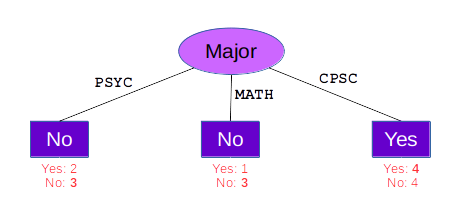
\includegraphics[width=0.6\textwidth]{majorOnTop.png}
\caption{A one-level decision tree if we put the \textsf{major} feature at the
root -- it would classify \textbf{ten} of the seventeen training points
correctly.}
\label{fig:majorOnTop}
\end{figure}

Let's repeat this analysis for the other two features and see if either one
fares any better. Here's the query for \textsf{age}:

\begin{Verbatim}[fontsize=\small,samepage=true,frame=single,framesep=3mm]
students.groupby('age').VG.value_counts()
\end{Verbatim}
\vspace{-.2in}

\begin{Verbatim}[fontsize=\small,samepage=true,frame=leftline,framesep=5mm,framerule=1mm]
age     VG 
middle  No     6
        Yes    2
old     Yes    2
        No     1
young   No     3
        Yes    3
Name: VG, dtype: int64
\end{Verbatim}

Making the sensible predictions at the leaves based on these values gives the
tree in Figure~\ref{fig:ageOnTop}. It gets \textbf{eleven} points right (65\%)
-- a bit of an improvement.

\begin{figure}[ht]
\centering
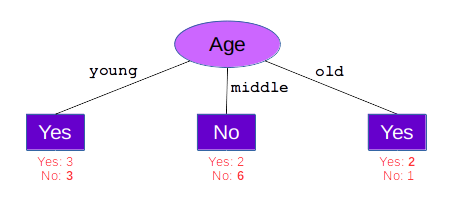
\includegraphics[width=0.6\textwidth]{ageOnTop.png}
\caption{A one-level decision tree if we chose the \textsf{age} feature for the
root -- it would classify \textbf{eleven} of the seventeen training points
correctly.}
\label{fig:ageOnTop}
\end{figure}

Finally, we could put \textsf{gender} at the root. Here's the query for it:

\begin{samepage}
\begin{Verbatim}[fontsize=\small,samepage=true,frame=single,framesep=3mm]
students.groupby('gender').VG.value_counts()
\end{Verbatim}
\vspace{-.2in}

\begin{Verbatim}[fontsize=\small,samepage=true,frame=leftline,framesep=5mm,framerule=1mm]
gender  VG 
F       No     8
        Yes    2
M       Yes    5
        No     1
O       No     1
Name: VG, dtype: int64
\end{Verbatim}
\end{samepage}

Paydirt! Splitting on the \textsf{gender} feature first, as shown in
Figure~\ref{fig:genderOnTop}, gets us a whopping \textbf{fourteen} points correct,
or over 82\%. This is clearly the winner, since we're being greedy and not
bothering to look further downstream anyway. So \textsf{gender} at the root it
is.

\begin{figure}[ht]
\centering
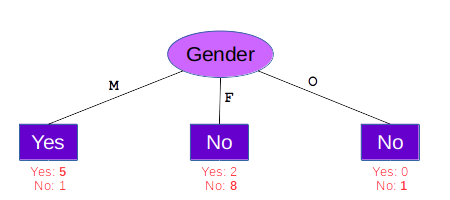
\includegraphics[width=0.6\textwidth]{genderOnTop.png}
\caption{A one-level decision tree if we chose the \textsf{gender} feature for
the root. It would classify \textbf{fourteen} of the seventeen training points
correctly -- easily the best of the three choices.}
\label{fig:genderOnTop}
\end{figure}

It's worth taking a moment to look at those \texttt{.value\_counts()} outputs
and see if you can develop some intuition about why \textsf{gender} worked so
much better at the root than the other two features. The reason is that for
this data set, \textsf{gender} split the data into groups that were more
\textbf{homogeneous} than the other splits gave. Homogeneous here means that
each group was more ``pure,'' or simply, more alike. \textsf{Gender} gave us a
5-to-1 lopsided ratio on the \texttt{M} branch, and an even more lopsided
2-to-8 ratio on the \texttt{F} branch. Intuitively, this means that
\textsf{gender} really is correlated with videogame use, and this shows up in
purer splits. Contrast this with the situation when we split on \textsf{major}
first, and we ended up with a yucky 4-to-4 ratio on the \texttt{CPSC} branch.
That's the worst of all possible worlds: learning someone's a Computer Science
major doesn't tell you jack about their videogame use, which means it's pretty
useless to split on.
%I love the word ``training'' for this, by the way.
